% last updated in April 2002 by Antje Endemann
% Based on CVPR 07 and LNCS, with modifications by DAF, AZ and elle, 2008 and AA, 2010, and CC, 2011; TT, 2014

\documentclass[runningheads]{llncs}
\usepackage{graphicx}
\usepackage{amsmath,amssymb} % define this before the line numbering.
\usepackage{ruler}
\usepackage{color}
\usepackage{subfigure}
\usepackage[width=122mm,left=12mm,paperwidth=146mm,height=193mm,top=12mm,paperheight=217mm]{geometry}
\begin{document}
% \renewcommand\thelinenumber{\color[rgb]{0.2,0.5,0.8}\normalfont\sffamily\scriptsize\arabic{linenumber}\color[rgb]{0,0,0}}
% \renewcommand\makeLineNumber {\hss\thelinenumber\ \hspace{6mm} \rlap{\hskip\textwidth\ \hspace{6.5mm}\thelinenumber}}
% \linenumbers
\pagestyle{headings}
\mainmatter
\def\ECCV14SubNumber{***}  % Insert your submission number here

\title{LKHT - Lukas-Kanade Hough-Transform for the detection of faces and their parts} % Replace with your title

\titlerunning{ECCV-14 submission ID \ECCV14SubNumber}

\authorrunning{ECCV-14 submission ID \ECCV14SubNumber}

\author{Anonymous ECCV submission}
\institute{Paper ID \ECCV14SubNumber}


\maketitle

%\begin{abstract}
%State-of-the-art approaches to face/object detection are based on exhaustively evaluating a set of discriminatively trained HOG templates over all possible locations in a given image using a sliding window approach. Although such approaches can accommodate for both rigid and deformable objects, in the latter case, object parts are allowed to score independently of the others while for the shape and appearance optimization to be efficient only loosely connected shape models are considered. In this paper, to alleviate these problems to some extend, we propose an object detection algorithm in which densely connected models of shape and appearance are jointly optimized using efficient Gauss-Newton optimization. Our approach differs from prior work in 3 aspects: (a) rather than exhaustively evaluating multiple templates to cope with pose or other deformations, our algorithm applies the Lukas-Kanade (LK) algorithm in order to evaluate the score of a \textit{single} deformable template in a sliding window fashion, (b) by capitalizing on the basin of attraction of the LK algorithm, we formulate a Hough-Transform voting scheme that rejects background and rewards image locations for which the LK algorithm converges to similar solutions, and (c) unlike most current approaches, our model is a generative one based on the principal components of HOG features. We have applied our method to the problem of detecting faces and their parts, and we report significant improvement over a state-of-the-art approach based on discriminatively trained deformable part models.
%\end{abstract}

\begin{abstract}
We propose a novel approach to face/object detection which we call Lukas-Kanade Hough-Transform. In particular, we firstly propose to employ the Lukas-Kanade (LK) algorithm in a \textit{sliding window} fashion to fit a deformable model, and use the ``goodness'' of the fit as a score to detect faces. Secondly, we propose to capitalize on the large basin of convergence of our LK algorithm to set up a Hough-Transform voting scheme for filtering out false positives caused by irrelevant objects/background, and boosting up the scores corresponding to real faces. In contrast to most work on face/object detection based on deformable parts models, we use a densely connected shape model and an appearance model which are \textit{jointly} optimized using an efficient Gauss-Newton algorithm. Our approach is largely motivated by recent gradient descent optimization approaches to facial feature detection, in which impressive results have been reported for ``in-the-wild'', unconstrained settings. Essentially, rather than using a face detector to initialize such methods, we instead propose to employ them in order to detect the location of a face in an image along with its parts. We have applied our method to the problem of detecting faces and their parts, and we report significant improvement over a state-of-the-art approach based on discriminatively trained deformable part models.

\end{abstract}


\section{Introduction}\label{S:I}

Object and face detection is one of the most popular and well-studied problems in computer vision with a multitude of approaches proposed over the last years reporting a varying degree of success. One of the most influential and successful approaches with impressive results being reported for the unconstrained, ``in-the-wild'' setting is the Dalal and Triggs object detector \cite{dalal2005histograms}, and the follow-up breakthrough of Deformable Part Models (DPMs) \cite{felzenszwalb2005pictorial, felzenszwalb2010object}. Such algorithms are based on HOG object templates discriminatively trained using SVMs and capitalize on the increasing availability of large labelled training sets to report excellent performance for difficult object detection and part localization problems.

Very often, and in particular for the problem of analyzing faces, such algorithms are used to initialize part localization techniques like Active Appearance Models \cite{cootes2001active, matthews2004active} and Constrained Local Models \cite{cristinacce2008automatic,saragih2011deformable}. For objects like faces such algorithms have been shown to largely outperform (see for example \cite{asthana2013robust}) DPMs. More recently gradient descent optimization approaches to facial feature detection \cite{xiongsupervised, tzimiropoulosoptimization}) have reported impressive results for ``in-the-wild'', unconstrained settings. In this paper, rather than using HOG templates to initialize such methods, we propose to employ them in order to detect the location of a face in an image along with its parts.

\textbf{Object detection.} We start by summarizing the Dalal and Triggs approach and DPMs which are the prevalent approaches to object/face detection. A HOG object template $\mathbf{T}$ is typically expressed as a $w \times h$ array of $N_f-$dimensional feature vectors. To learn a HOG template for an object class, one first needs to extract arrays with HOG descriptors from a set of training images for that class (typically annotated with bounding boxes that indicate the location of the objects`), as well as from negative examples randomly selected from the background. A HOG descriptor is a feature vector of size $N_f$ extracted from a $N_s \times N_s$ image region (typically, $N_f=36$ and $N_s=8$). Finally, a HOG template is learned discriminately by feeding the extracted HOG features to a linear SVM classifier. The resulting template is aimed to capture the visual appearance of an object class and can be interpreted as filter which is tuned to peak only when it is correlated with HOG features from objects of the same class, and hence of similar appearance.

To detect an object in an image $\mathbf{I}$, one needs to exhaustively evaluate $\mathbf{T}$ over a grid $G$ of image locations usually in a sliding window fashion. Let us denote by $\mathbf{x} = [x, \; y]^T$ a point on the grid, and by $\mathbf{H}_I(\mathbf{x})$ the array of HOG features extracted at location $\mathbf{x}$ of image $\mathbf{I}$. Then, an object is detected if there is one or more image locations for which the score surface
\begin{equation}
\textrm{Score}_A(\mathbf{x}) = \mathbf{T}^T \mathbf{H}_I(\mathbf{x}), \;\;\; \mathbf{x} \in G, \label{E:S}
\end{equation}
is greater than threshold. $\textrm{Score}_A$ measures the similarity of the HOG template and the appearance of HOG features extracted at location $\mathbf{x}.$ 

Although (\ref{E:S}) can be very efficiently implemented with using fast convolution routines, unfortunately a single template is not sufficient for most applications. In particular, to enable the detection of objects in different scales, one needs to extract HOG features from $\mathbf{I}$ at multiple scales S, hence the score surface becomes a function of the scale
\begin{equation}
\textrm{Score}_A(\mathbf{x}, s) = \mathbf{T}^T \mathbf{H}_I(\mathbf{x}, s), \;\;\; \mathbf{x} \in G, \; s \in S. \label{E:S1}
\end{equation}   
To accommodate for changes in viewpoint, we can train a mixture of templates, one for each viewpoint$v$. In this case the score becomes
\begin{equation}
\textrm{Score}_A(\mathbf{x}, s, v) = \mathbf{T}(v)^T \mathbf{H}_I(\mathbf{x}, s), \;\;\; \mathbf{x} \in G, \; s \in S, \; v \in V, \label{E:S2}
\end{equation}
where $\mathbf{T}(v)$ is the template trained for viewpoint $v$. 

Recently, multi-view rigid HOG templates have been shown to perform remarkably well for face detection in \cite{ramanan2011}. Much better results were obtained though when the face was described as rigid template (root) $\mathbf{T}_i$ along with a collection of HOG part templates $\mathbf{T}_i$ which are allowed to deform according to a shape model \cite{felzenszwalb2005pictorial, felzenszwalb2010object}. In particular, the total score is given by
\begin{equation}
\textrm{Score} = \sum_i\textrm{Score}_A(i) + \textrm{Score}_S(\mathbf{z}), \label{E:DPM}
\end{equation}
where $\mathbf{z}$ is a configuration of parts and $\textrm{Score}_S(\mathbf{z})$ is the score for this configuration. $\textrm{Score}_S$ is used to penalize unlikely configurations which for some reason could happen to produce high values for the appearance term. Note that there are mainly two problems arising from the formulation of (\ref{E:DPM}): (a) parts are allowed to score independently of each other, and (b) the shape model is assumed to be a tree, which is often too loose especially for objects like faces. On the other hand, the best location of the parts with respect to the root can be efficiently found using dynamic programming and distance transforms \cite{felzenszwalb2010object}, i.e. (\ref{E:DPM}) is globally optimizable. 

In \cite{felzenszwalb2010object}, the shape model is a star model learned from positives examples annotated with bounding boxes only, using a latent SVM approach. More recently, the authors of \cite{ramanan2011} have shown that impressive performance for the problem of face detection and part localization can be obtained, if one builds the shape model in a supervised way by using manual annotations of parts. Although the authors report excellent results for the problem of face detection, the localization of parts is often less accurate. One drawback of \cite{ramanan2011} is that the best performance is obtained by using different mixtures of models for handing pose and facial expression resulting in very large number of part HOG templates, although this is addressed to some extend by follow-up work \cite{pirsiavash2012steerable}. We also refer the reader to \cite{yupose} for an interesting extension of \cite{ramanan2011}.

\textbf{Main results.} In this paper, to address some of the aforementioned problems (in particular problems (a) and (b)), we propose a novel approach to face/object detection which we call Lukas-Kanade Hough-Transform. In particular, we propose to employ the Lukas-Kanade (LK) algorithm in a \textit{sliding window} fashion to fit a deformable model, and use the ``goodness'' of the fit as a score to detect faces. Secondly, we propose to capitalize on the large basin of convergence of our LK algorithm to set up a Hough-Transform voting scheme filtering out false positives caused by irrelevant objects/background, and boosting up the scores corresponding to real faces. In contrast to most work on face/object detection based on deformable parts models (e.g. \cite{felzenszwalb2010object, ramanan2011}), we use a densely connected shape model and an appearance model which are \textit{jointly} optimized using an efficient Gauss-Newton algorithm. Our approach is largely motivated by recent gradient descent optimization approaches to facial feature detection \cite{xiongsupervised, tzimiropoulosoptimization}), in which impressive results have been reported for ``in-the-wild'', unconstrained settings. In particular, our approach differs from the deformable part model formulation of (\ref{E:DPM}) in 3 important aspects:
\begin{itemize}
\item
Rather than exhaustively evaluating multiple templates as in (\ref{E:DPM}) in order to cope with pose or other deformations, we propose to employ the Lukas-Kanade (LK) algorithm in a \textit{sliding window} fashion in order to evaluate the score of a \textit{single} deformable template over a grid of image locations. In particular, as deformable template, we choose an Active Appearance Model, i.e. a densely connected shape model and an appearance model which deforms according to a piece-wise affine motion model. We fit this model using an efficient Gauss-Newton algorithm \cite{matthews2004active}, the complexity of which is only $O(nN)$ per iteration, where $N$ is the number of features in the appearance model, and $n$ is the size of the shape model (only, 7 in our model). We note however that other gradient descent optimization approaches (e.g. \cite{xiongsupervised}) could be possibly employed.
\item 
We capitalize on the basin of attraction of the LK algorithm and formulate a Hough-Transform voting scheme that filters out irrelevant objects and background areas, whilst at the same ``rewards'' candidate image locations for which the LK algorithm converges to similar solutions. The main idea here is that if the Gauss Newton algorithm converges to the same solution for multiple initializations, then the converged solution ``must'' be a face.
\item 
Unlike most current approaches, our appearance model is a generative one, and in particular, in order to enforce a large basin of attraction for our voting scheme, we propose to build it by applying Principal Components Analysis on SIFT features \cite{lowe2004distinctive}.
\end{itemize}
We have applied our method to the problem of detecting faces and their parts, and we report significant improvement over the state-of-the-art approach of \cite{ramanan2011}.


\begin{figure*}[t!]
\centering
\subfigure[Selected fitted shapes and associated votes.]{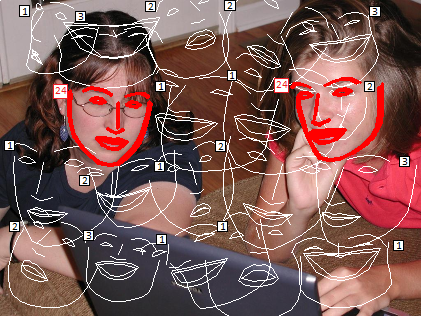
\includegraphics[width=0.4\columnwidth]{images/image.png}}\\
\subfigure[Votes.]{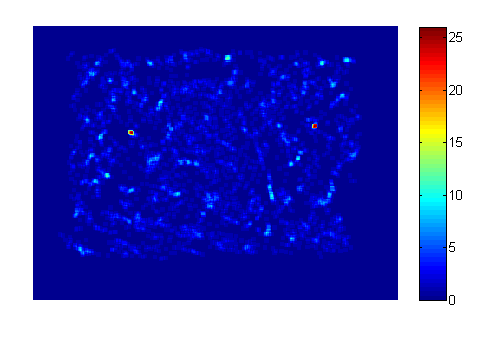
\includegraphics[width=0.4\columnwidth]{images/so_votes.png}}\\
\subfigure[Normalised correlation score (max.).]{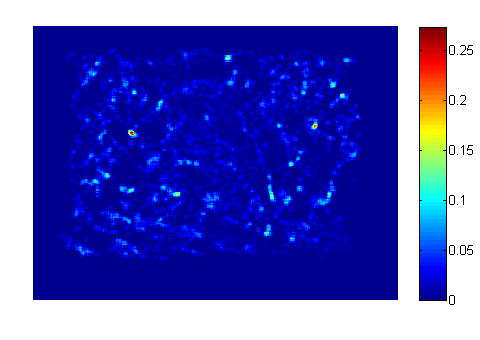
\includegraphics[width=0.4\columnwidth]{images/so_cormax.png}}\\
\subfigure[Normalised correlation score weighted by votes.]{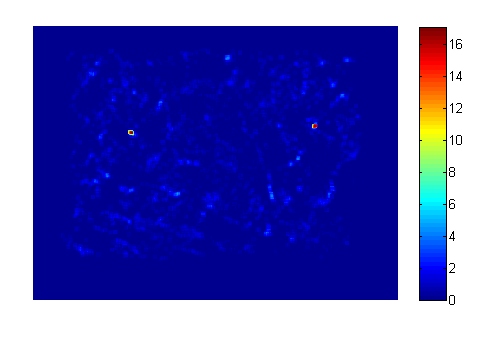
\includegraphics[width=0.4\columnwidth]{images/so_cor.png}}
\caption{Overview of our system.}
\label{F:SO}
\end{figure*}

\section{System Overview} \label{S:Overview}

Our system scans an image in a sliding window fashion and for each location $\mathbf{x}$ (we used a grid of equally spaced points), it fits an Active Appearance Model (AAM) using the Lukas-Kanade (LK) algorithm, and measures the ``goodness'' of the fit. Image locations that converge to the same location cast votes for that location in a fashion similar to Hough Transform. Fig. \ref{F:SO} aims to provide an overview of our approach. Its main components are analyzed as follows

\textbf{AAM fitting with LK.} An advantage of the AAM formulation is that shape and appearance can be compactly represented by a small number of parameters. In particular, our AAM has $n=7$ shape parameters which control similarity transforms and additionally capture basic shape deformations due to pose and expressions. Note that, in contrast to the DPM approach of \cite{ramanan2011}, $n$ is not a function of the number of parts which is usually much larger (68 in our case). Our AAM has additionally $m$ appearance parameters (25 in our case) which control the appearance variation of ``SIFT-Faces'' (please see Section \ref{S:Models} for more details). 

Fitting an AAM to a new image entails estimating the model parameters so that a model instance is ``close enough'' (typically in a least-squares sense) to the given image. This can be formulated as a non-linear least-squares problem which is typically solved using iterative methods. State-of-the-art methods for AAM fitting are based on analytic gradient descent and, in particular, on extensions of the Lukas-Kanade algorithm based on Gauss-Newton optimization. Although exact AAM fitting using Gauss-Newton has a cost $O(nmN + n^2N)$ per iteration, where $N$ is the number of features in the SIFT eigenvectors \cite{tzimiropoulosoptimization}, one can solve an approximate Gauss-Newton problem efficiently in $O(nN)$ \cite{matthews2004active}. Our parallel implementation of this algorithm can fit a face at more than 1000 FPS. This enables us to use it to scan an image in a few seconds.

\textbf{Scoring faces via reconstruction error.} Once an AAM fitting procedure converges, we can measure the ``goodness'' of the fit by measuring the normalized correlation (so that values are between -1 and 1) between the model instance and the candidate face extracted from the given image. This has a cost $O(mN)$. Note that this generative approach has been recently shown to produce state-of-the-art results for the problem of face recognition \cite{naseem2010linear, zhang2011sparse}. We extend it here to allow for deformable templates (i.e. AAMs) built from SIFT features, and show that it can be also applied for detection (as opposed to recognition).

\textbf{Lukas Kanade Hough-Transform voting.} Although one detect via just looking at the maximum values 


%Its use for face detection goes back to the seminal work of ``Eigenfaces'' \cite{turk1991eigenfaces}. Three notable %differences between our scoring approach and \cite{turk1991eigenfaces} are that (a) in our approach facial appearance %is measured



\bibliographystyle{splncs}
\bibliography{face_bibtex_n}
\end{document}
